\doclearpage
\section{String Toolbox}
\label{sec:string-toolbox}

We present a collection of protocols that serve as building blocks for the string-matching protocols of later sections, and that can be reused elsewhere as well.

\subsection{Broadcast Check}
\label{sec:broadcast}

In some protocols, we need to expand a string-level column into a character-level one by copying each string's entry onto all of its characters; we call this operation \emph{broadcasting}; \cref{fig:broadcast-example} shows a small example.
\begin{figure}[H]
\centering
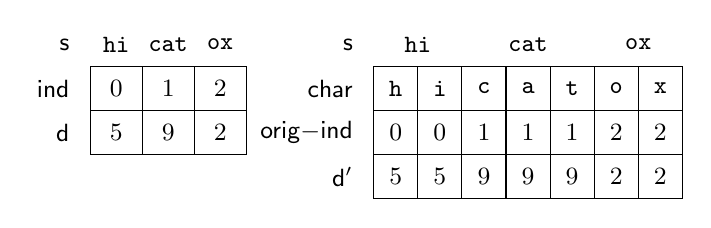
\begin{tikzpicture}[x=1cm, y=1cm,
    cell/.style={draw, minimum size=5.6mm, inner sep=0pt, font=\small},
    rowlab/.style={font=\small, anchor=east},
    hd/.style={font=\small\ttfamily}]
  % ---- string-level columns ----
  \node[rowlab] at (0,0.56)  {$\mathsf{s}$};
  \node[rowlab] at (0,0)     {$\mathsf{ind}$};
  \node[rowlab] at (0,-0.56) {$\mathsf{d}$};
  \foreach \i/\s/\d in {0/hi/5, 1/cat/9, 2/ox/2}{
    \node[hd]   at (0.47+\i*0.66, 0.56)  {\s};
    \node[cell, minimum width=6.6mm] at (0.47+\i*0.66, 0)     {\i};
    \node[cell, minimum width=6.6mm] at (0.47+\i*0.66, -0.56) {\d};
  }
  % ---- character-level columns ----
  \begin{scope}[xshift=3.6cm]
  \node[rowlab] at (0,0.56)  {$\mathsf{s}$};
  \node[rowlab] at (0,0)     {$\mathsf{char}$};
  \node[rowlab] at (0,-0.56) {$\mathsf{orig\text{-}ind}$};
  \node[rowlab] at (0,-1.12) {$\mathsf{d}^\prime$};
  \node[hd] at (0.70,0.56) {hi};
  \node[hd] at (2.10,0.56) {cat};
  \node[hd] at (3.50,0.56) {ox};
  \foreach \j/\c/\o/\d in {0/h/0/5, 1/i/0/5, 2/c/1/9, 3/a/1/9, 4/t/1/9, 5/o/2/2, 6/x/2/2}{
    \node[cell, font=\small\ttfamily] at (0.42+\j*0.56, 0) {\c};
    \node[cell] at (0.42+\j*0.56, -0.56) {\o};
    \node[cell] at (0.42+\j*0.56, -1.12) {\d};
  }
  \end{scope}
\end{tikzpicture}
\caption{Broadcasting the string-level column $\mathsf{d} = (5, 9, 2)$ of the strings \texttt{hi}, \texttt{cat} and \texttt{ox} onto their characters yields the character-level column $\mathsf{d}^\prime$.}
\label{fig:broadcast-example}
\end{figure}
 More formally, a character-level column $\mathsf{d}^\prime$ is the broadcast of a string-level column $\mathsf{d}$: every character carries the entry of the string it belongs to, $\mathsf{d}^\prime[c] = \mathsf{d}[\mathsf{orig\text{-}ind}[c]]$. The following PIOP checks this relation.
\begin{DefinePIOP}{Broadcast Check}{broadcast}
  \emph{Inputs:} a string column $\Oracle{\MLE{\strcol}}$ with all of its main and auxiliary oracles; a string-level column $\Oracle{\MLE{\mathsf{d}}}$ and its claimed broadcast, the character-level column $\Oracle{\MLE{\mathsf{d}'}}$.
  \begin{enumerate}[nosep]
    \item (\emph{Parse}) $\PIOPProver$ and $\PIOPVerifier$ parse $\Oracle{\MLE{\strcol}}$ to obtain the origin-index oracle $\Oracle{\MLE{\mathsf{orig\text{-}ind}}}$.
    \item $\PIOPVerifier$ samples a random $r \samples \F$ and sends it to $\PIOPProver$.
    \item $\PIOPProver$ and $\PIOPVerifier$ invoke \cref{piop:lookup-check} on $(\mathbf{1},\, \mathsf{orig\text{-}ind} + r\,\mathsf{d}') \lookup (\mathbf{1},\, \mathsf{ind} + r\,\mathsf{d})$.
  \end{enumerate}
\end{DefinePIOP}
The formal definition and security proofs are deferred to \cref{sec:proof-bcast}. 

\subsection{Consistency-Checking protocols}
\label{sec:consistency-checking}
The auxiliary columns must remain trusted and in sync with one another and with the main column at all times. Since the prover is untrusted, it cannot update them freely and every update must come with a proof of well-formedness. We therefore design protocols that prove this well-formedness.

Three kinds of updates arise in the system: \emph{data-preserving} (\cref{sec:data-preserving}), \emph{domain-preserving} (\cref{sec:domain-preserving}) and \emph{domain-altering}. The relational core of SQL falls almost entirely into the first two, with the third one confined to a handful of value-constructing expressions where all of the columns are freshly materialized and new strings are introduced: aggregates such as \texttt{STRING\_AGG}, and string constructors such as \texttt{CONCAT}, \texttt{SUBSTRING}, case mapping, casts, and literals.

\subsubsection{Data-Preserving Update}
\label{sec:data-preserving}
In a data-preserving update, \emph{only the activators} are freshly materialized, i.e. columns $\mathsf{a}$ and $\mathsf{char\text{-}act}$, while the remaining data columns are inherited unchanged. These are the operators that merely re-mark which rows are active; such as selection, projection, \texttt{DISTINCT}, and \texttt{LIMIT}.

Before relying on the new activators, the verifier must confirm that the two activators are \emph{consistent}. \Cref{fig:consistency-example} shows a consistent and an inconsistent update.
\begin{figure}[H]
\centering
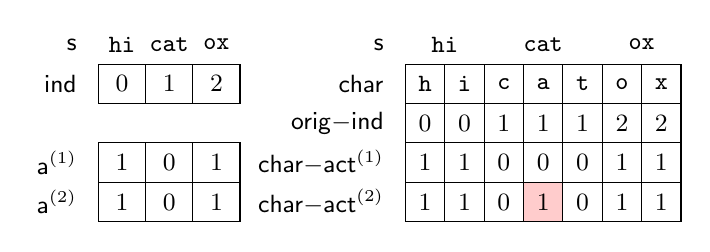
\begin{tikzpicture}[x=1cm, y=1cm,
    cell/.style={draw, minimum size=5mm, inner sep=0pt, font=\small},
    bad/.style={fill=red!20},
    rowlab/.style={font=\small, anchor=east},
    hd/.style={font=\small\ttfamily}]
  % ---- string-level columns ----
  \node[rowlab] at (0,0.5)  {$\mathsf{s}$};
  \node[rowlab] at (0,0)    {$\mathsf{ind}$};
  \node[rowlab] at (0,-1.0) {$\mathsf{a}^{(1)}$};
  \node[rowlab] at (0,-1.5) {$\mathsf{a}^{(2)}$};
  \foreach \i/\s/\x/\y in {0/hi/1/1, 1/cat/0/0, 2/ox/1/1}{
    \node[hd]   at (0.45+\i*0.6, 0.5)  {\s};
    \node[cell, minimum width=6mm] at (0.45+\i*0.6, 0)    {\i};
    \node[cell, minimum width=6mm] at (0.45+\i*0.6, -1.0) {\x};
    \node[cell, minimum width=6mm] at (0.45+\i*0.6, -1.5) {\y};
  }
  % ---- character-level columns ----
  \begin{scope}[xshift=3.9cm]
  \node[rowlab] at (0,0.5)  {$\mathsf{s}$};
  \node[rowlab] at (0,0)    {$\mathsf{char}$};
  \node[rowlab] at (0,-0.5) {$\mathsf{orig\text{-}ind}$};
  \node[rowlab] at (0,-1.0) {$\mathsf{char\text{-}act}^{(1)}$};
  \node[rowlab] at (0,-1.5) {$\mathsf{char\text{-}act}^{(2)}$};
  \node[hd] at (0.65,0.5) {hi};
  \node[hd] at (1.90,0.5) {cat};
  \node[hd] at (3.15,0.5) {ox};
  \foreach \j/\c/\o/\x/\y/\st in {0/h/0/1/1/cell, 1/i/0/1/1/cell, 2/c/1/0/0/cell, 3/a/1/0/1/bad, 4/t/1/0/0/cell, 5/o/2/1/1/cell, 6/x/2/1/1/cell}{
    \node[cell, font=\small\ttfamily] at (0.4+\j*0.5, 0) {\c};
    \node[cell] at (0.4+\j*0.5, -0.5) {\o};
    \node[cell] at (0.4+\j*0.5, -1.0) {\x};
    \node[cell, \st] at (0.4+\j*0.5, -1.5) {\y};
  }
  \end{scope}
\end{tikzpicture}
\caption{Two data-preserving updates that deactivate the string \texttt{cat}. Update~(1) is consistent: every character carries the activator bit of its string. Update~(2) is not: the character \texttt{a} of the inactive string \texttt{cat} remains active (shaded).}
\label{fig:consistency-example}
\end{figure}

To prove that the update was done correctly, it suffices to show that both columns are boolean, using \cref{piop:boolean-check}, and every character inherits the active bit of the string it belongs to. To prove the inheritance condition, we need to prove that if a string identified by index $i$ has length $m$, then there are $m$ active characters belonging to index $i$. Viewing the character-level columns as a table $\mathsf{Chars}$ with columns $\mathsf{orig\text{-}ind}$ and $\mathsf{char\text{-}act}$, and the string-level columns as a table $\mathsf{Strs}$ with columns $\mathsf{ind}$ and $\mathsf{l}$ and activator $\mathsf{a}$, this exactly translates to the following check using a \texttt{SUM GROUP BY} query:
\begin{equation}\label{eq:cons-groupby}
\begin{array}{@{}l@{}}
\sqlline{\sqlkw{SELECT} orig\_ind,}\\
\sqlline{\ \ \ \ \ \ \ \sqlkw{SUM}(char\_act)}\\
\sqlline{\ \ \sqlkw{FROM} Chars}\\
\sqlline{\ \sqlkw{GROUP BY} orig\_ind;}
\end{array}
=
\begin{array}{@{}l@{}}
\sqlline{\sqlkw{SELECT} ind, l}\\
\sqlline{\ \ \sqlkw{FROM} Strs;}
\end{array}
\end{equation}
$\truthtable$~\cite{cryptoeprint:2026/1260} proves a \texttt{SUM GROUP BY} with a single \cref{piop:keyedsumcheck}, and we reuse that protocol verbatim.
\begin{DefinePIOP}{Data-Preserving Update Check}{data-preserving-update-check}
  \emph{Inputs:} The updated string column $\Oracle{\MLE{\strcol}}$ with all of its main and auxiliary oracles.
  \begin{enumerate}[nosep]
    \item (\emph{Parse}) $\PIOPProver$ and $\PIOPVerifier$ parse $\Oracle{\MLE{\strcol}}$ to obtain the activator oracles $\Oracle{\MLE{\mathsf{a}}}$ and $\Oracle{\MLE{\mathsf{char\text{-}act}}}$, the origin-index oracle $\Oracle{\MLE{\mathsf{orig\text{-}ind}}}$, and the length oracle $\Oracle{\MLE{\mathsf{l}}}$.
    \item (\emph{booleanity}) To check if the updated activator is boolean, $\PIOPProver$ and $\PIOPVerifier$ invoke \cref{piop:boolean-check} on $\mathsf{char\text{-}act}$ and on $\mathsf{a}$.
    \item (\emph{activator consistency}) To check \cref{eq:cons-groupby}, $\PIOPProver$ and $\PIOPVerifier$ invoke \cref{piop:keyedsumcheck} on $\mathsf{Chars}$ and $\mathsf{Strs}$, which forces $\sum_{j:\,\mathsf{orig\text{-}ind}[j]=i}\mathsf{char\text{-}act}[j] = \mathsf{a}[i]\cdot\mathsf{l}[i]$ for every key $i$.
  \end{enumerate}
\end{DefinePIOP}
The formal definition and the security proofs are deferred to \cref{sec:proof-cons}.

\subsubsection{Domain-Preserving Update}
\label{sec:domain-preserving}

In a domain-preserving update, all of the main and auxiliary columns, including data and activators, are freshly materialized by the untrusted prover, yet every output string cell is a copy of some input cell, so no new string is introduced. This covers all join types, \texttt{UNION}, \texttt{INTERSECT}, \texttt{EXCEPT}, sorting, and value-selecting aggregates such as \texttt{MIN}, \texttt{MAX}, and \texttt{ANY\_VALUE}.


Since the prover freshly materializes every new column, the check must establish two things: that the new columns form a well-formed arithmetization, and that no new string is introduced. For the second property we exploit the fact that, although the column is fresh, its strings are not: each of them already appears in a string column committed by the data owner. The prover therefore points each new string to a source string in that column, and we check that the two agree on every attribute of the arithmetization, namely the hash, the length, the rank, and the sequence of characters.

The pointers form the \emph{source column} $\mathsf{src}$: a string-level column of the new table in which $\mathsf{src}[i]$ is the index of the row of the old column that row $i$ was copied from. Some operators produce this column as a by-product of their own proof, in which case it is already trusted and is passed to the check; otherwise the prover supplies it, and the lookups below are what make it trustworthy. The check also uses the \emph{index column} $\mathsf{ind} = (0, 1, \dots, N-1)$, the evaluation table of the index polynomial $\idx_\mu$ of \cref{sec:prelims}, which numbers the rows of the old column so that $\mathsf{src}$ can be matched against it.

\ali{Too many polynomials}
\ali{add intuition before the box and link it in the piop}

\begin{DefinePIOP}{Full String Validity Check}{full-str-valid}
  \emph{Inputs:} the input column $\strcol^{\mathsf{old}}$ and the output column $\strcol^{\mathsf{new}}$, each with all of its main and auxiliary oracles (\cref{sec:string-arith}); $\Oracle{\MLE{\mathsf{ind}}}$; and optionally a trusted source column $\Oracle{\MLE{\mathsf{src}}}$.
  \begin{enumerate}[nosep]
    \item \emph{(Activators and lengths)} $\PIOPProver$ and $\PIOPVerifier$ invoke \cref{piop:data-preserving-update-check} on $\strcol^{\mathsf{new}}$, establishing $\NPRelation_{\mathsf{Cons}}$ for the new activator pair.
    \item \emph{(Offset enumeration)} $\PIOPVerifier$ samples $r \samples \F$ and sends it to $\PIOPProver$; the parties then invoke \cref{piop:nodup-check} on a column with data $\mathsf{orig\text{-}ind^{new}} + r\,\mathsf{int\text{-}ind^{new}}$ and activator $\mathsf{char\text{-}act^{new}}$.
    \item \emph{(Source column)} If no trusted source column is given a priori, $\PIOPProver$ sends $\Oracle{\MLE{\mathsf{src}}}$ to $\PIOPVerifier$.
    \item \emph{(String-level provenance)} $\PIOPProver$ and $\PIOPVerifier$ invoke \cref{piop:lookup-check} on the statement $(\mathsf{src}, \mathsf{h}^{\mathsf{new}}, \mathsf{l}^{\mathsf{new}}, \mathsf{rk}^{\mathsf{new}}, \mathsf{a}_h^{\mathsf{new}}) \lookup (\mathsf{ind}, \mathsf{h}^{\mathsf{old}}, \mathsf{l}^{\mathsf{old}}, \mathsf{rk}^{\mathsf{old}}, \mathsf{a}_h^{\mathsf{old}})$, so every new row inherits the hash, length and rank of its source row.
    \item \emph{(Character-level provenance)}\label[step]{full-str:char-lookup} $\PIOPProver$ sends the broadcast $\Oracle{\MLE{\mathsf{src}^\prime}}$ of $\mathsf{src}$ onto the characters, which the parties check with \cref{piop:broadcast}, and then invoke \cref{piop:lookup-check} on the statement $(\mathsf{src}^\prime, \mathsf{char}^{\mathsf{new}}, \mathsf{int\text{-}ind}^{\mathsf{new}}) \lookup (\mathsf{orig\text{-}ind}^{\mathsf{old}}, \mathsf{char}^{\mathsf{old}}, \mathsf{int\text{-}ind}^{\mathsf{old}})$.
  \end{enumerate}
\end{DefinePIOP}




\subsection{Length Filtering}
\label{sec:length-filtering}

Length filtering discards every string shorter than a threshold $k$, keeping only those of length at least $k$. This is the pruning needed in pattern matching: in every filter  a string can match only if it is at least as long as the pattern, so any shorter string is a guaranteed non-match and can be removed before the filter runs. As we will see in \cref{sec:multi-char-pattern-matching}, this is not merely an optimization: length filtering is necessary for the pattern-matching protocols to remain complete and sound. The length filtering relation $\NPRelation_{\mathsf{LenFilter}}$, stated in \cref{sec:proof-lenfilter}, takes the threshold $k$ as instance and requires that the new string-level activator $\mathsf{a}^\prime$ keep exactly the active strings of length at least $k$, and that the new character-level activator $\mathsf{char\text{-}act}^\prime$ keep exactly the characters of the kept strings. The following PIOP checks this relation.

\begin{DefinePIOP}{Length Filtering Check}{len-filter}
  \emph{Inputs:} $\Oracle{\MLE{\mathsf{orig\text{-}ind}}}, \Oracle{\MLE{\mathsf{l}}}, \Oracle{\MLE{\mathsf{a}}}, \Oracle{\MLE{\mathsf{char\text{-}act}}}$, threshold $k$.
  \begin{enumerate}[nosep]
    \item (\textit{Activator Update Validity}) $\PIOPProver$ and $\PIOPVerifier$ invoke \cref{piop:data-preserving-update-check} on the updated column $\strcol'$, whose activators are $\mathsf{a'}$ and $\mathsf{char\text{-}act'}$.
    \item (\textit{Containment}) $\PIOPProver$ and $\PIOPVerifier$ invoke \cref{piop:zerocheck} on the column $\mathsf{a'}\cdot(1-\mathsf{a})$.
    \item(\textit{False negative check}) $\PIOPProver$ and $\PIOPVerifier$ invoke the Negative \cref{piop:sign-check} on the column $(\mathsf{a}\cdot(1-\mathsf{a'}), \mathsf{l}-k)$.
    \item (\textit{False Positive check}) $\PIOPProver$ and $\PIOPVerifier$ invoke the Non-Negative \cref{piop:sign-check} on the column $(\mathsf{a'}, \mathsf{l}-k)$.
  \end{enumerate}
\end{DefinePIOP}


\subsection{Character Projection}
\label{sec:char-projection}

Several protocols need to look at the strings of a column ``one position at a time'': the lexicographic-ordering protocols of \cref{sec:lex-order} compare all strings on their first character, then on their second, and so on. We therefore need, for a position $k$, a \emph{string-level} column holding the $k$-th character of every string. Strings shorter than $k+1$ have no such character; following \cref{sec:sql-string-order}, we fill in the sentinel $\bot := -1$ there, which is smaller than every character code and thereby makes shorter strings sort first. We call this column the \emph{projection} of the string column onto position $k$. The projection relation $\NPRelation_{\mathsf{Proj}}$, stated in \cref{sec:proof-proj}, takes the position $k$ as instance and requires, for every active string $i$, that $\mathsf{c}_k[i]$ be the character of string $i$ at internal index $k$ if $\mathsf{l}[i] > k$, and the sentinel $\bot$ otherwise; in other words, $\mathsf{c}_k[i] = \pad{s_i}[k]$ is the $k$-th entry of the padded string of \cref{sec:sql-string-order}.

The check has three parts. The prover first splits the active strings into those long enough to have a $k$-th character and those that are not, by sending a boolean \emph{length indicator} $\mathsf{g}_k$ with $\mathsf{g}_k[i] = \mathbf{1}[\mathsf{l}[i] > k]$; two sign checks on $\mathsf{l} - k$, a $\mathsf{Pos}$ one where $\mathsf{g}_k = 1$ and a $\mathsf{NonPos}$ one where $\mathsf{g}_k = 0$, pin it down. For the long strings, the triple $(i, k, \mathsf{c}_k[i])$ must appear among the character-level triples $(\mathsf{orig\text{-}ind}[j], \mathsf{int\text{-}ind}[j], \mathsf{char}[j])$ of the active characters, which a \cref{piop:lookup-check} on random linear combinations of the triples enforces; since the active pairs $(\mathsf{orig\text{-}ind}[j], \mathsf{int\text{-}ind}[j])$ are distinct in a well-formed arithmetization (\cref{sec:domain-preserving}), membership pins $\mathsf{c}_k[i]$ to the unique character at that position. For the short strings, a \cref{piop:zerocheck} forces the sentinel.

\begin{DefinePIOP}{Character Projection Check}{char-proj}[Character Projection Check]
  \emergencystretch=3em\relax
  \emph{Inputs:} position $k$; the oracles $\Oracle{\MLE{\mathsf{char}}}, \Oracle{\MLE{\mathsf{orig\text{-}ind}}}, \Oracle{\MLE{\mathsf{int\text{-}ind}}},\allowbreak \Oracle{\MLE{\mathsf{char\text{-}act}}}, \Oracle{\MLE{\mathsf{l}}}, \Oracle{\MLE{\mathsf{a}}}, \Oracle{\MLE{\mathsf{ind}}}$; and the projection $\Oracle{\MLE{\mathsf{c}_k}}$.
  \vspace{2mm}
  \begin{enumerate}[nosep]
    \item (\emph{Length indicator})\label[step]{cp:len} $\PIOPProver$ sends $\Oracle{\MLE{\mathsf{g}_k}}$ with $\mathsf{g}_k[i] := \mathsf{a}[i] \mult \mathbf{1}[\mathsf{l}[i] > k]$. $\PIOPProver$ and $\PIOPVerifier$ invoke \cref{piop:boolean-check} on $\mathsf{g}_k$, \cref{piop:zerocheck} on $\mathsf{g}_k \mult (1 - \mathsf{a})$, the $\mathsf{Pos}$ \cref{piop:sign-check} on the column $(\mathsf{g}_k,\ \mathsf{l} - k)$, and the $\mathsf{NonPos}$ \cref{piop:sign-check} on the column $(\mathsf{a} \mult (1 - \mathsf{g}_k),\ \mathsf{l} - k)$.
    \item (\emph{Present characters})\label[step]{cp:present} $\PIOPVerifier$ samples $r \samples \F$ and sends it to $\PIOPProver$. $\PIOPProver$ and $\PIOPVerifier$ invoke \cref{piop:lookup-check} on
    $(\mathsf{g}_k,\ \mathsf{ind} + r\,k + r^2\,\mathsf{c}_k) \lookup (\mathsf{char\text{-}act},\ \mathsf{orig\text{-}ind} + r\,\mathsf{int\text{-}ind} + r^2\,\mathsf{char})$.
    \item (\emph{Absent characters})\label[step]{cp:absent} $\PIOPProver$ and $\PIOPVerifier$ invoke \cref{piop:zerocheck} on $\mathsf{a} \mult (1 - \mathsf{g}_k) \mult (\mathsf{c}_k + 1)$.
  \end{enumerate}
\end{DefinePIOP}

\parhead{Batching across positions}
When projections onto several positions $k_1, \dots, k_R$ are needed, as in \cref{piop:lex-sorted-check}, the $R$ lookups of \cref{cp:present} share the same right-hand side and can be merged into a single \cref{piop:lookup-check} whose left-hand side is the concatenation of the $R$ projected columns, so the character-level columns are swept once rather than $R$ times.
